\chapter{排列与组合~~二项式定理}
\section{排列与组合}
\subsection{加法原理和乘法原理}
假如我们要从甲地到乙地,可以乘火车、轮船或公共汽车,火车每天有两班,轮船有两班,公共汽车有六班,问从甲地到乙地有多少种不同的方法?

因为,从甲地到乙地,乘火车有两种不同的方法,乘轮船有两种不同的方法,乘公共汽车有六种不同的方法.而每种方法都可以由甲地到达乙地,因为,从甲地到乙地共有
$2+2+6=10$
种不同的方法.

一般地说,有如下原理:
\begin{blk}{加法原理}
如果完成某件事有$n$种方式,在第一种方式中有$m_1$种方法,在第二种方式中有$m_2$种方法……,在第$n$种方式中有$m_n$种方法. 那么完成这件事共有$m_1+m_2+\cdots+m_n$种不同的方法.
\end{blk}

又假如,要从甲地到丙地,必须经过乙地,现在已知由甲地到乙地有三条道路,由乙地到丙地有两条道路(图2.1),问从甲地到丙地共有多少种不同的走法?
\begin{figure}[htp]
    \centering
\begin{tikzpicture}
\node[draw, circle] (A) at (0,0){甲};    
\node[draw, circle] (B) at (4,0){乙};    
\node[draw, circle] (C) at (8,0){丙};
\draw(A)--(B);
\draw(A)to [bend left=45](B);
\draw(A)to [bend left=-45](B);
\draw(C)to [bend left=15](B);
\draw(C)to [bend left=-15](B);

\end{tikzpicture}
    \caption{}
\end{figure}

因为从甲地到乙地有3种不同的走法,到乙地后又各有两种不同的走法到丙地,因此,从甲地到丙地共有
$3\x2=6$
种不同的走法.

一般地说,有如下原理:

\begin{blk}
    {乘法原理}如果完成某种事需要分成$n$个步骤,第一步骤有$m_1$种方法,第二步骤有$m_2$种方法……,第$n$步骤有$m_n$种方法,那么完成这件事共有$m_1\cdot m_2\cdots m_n$种不同的方法.
\end{blk}

总的来说,如果完成一种事有几种不同的方法,这些方法又是互不相关的,任选一种方法都能完成这件事的,那么完成这件事的方法的总数,应该用加法计算. 如果完成一件事,必须分成若干步骤,每个步骤又有不同的方法,而且每一步骤中的一种方法完成之后,都可以开始下一步骤的工作,依次完成全部步骤,才能达到完成这一件事的目的,那么完成这件事的方法的总数应该用乘法计算.

\begin{ex}
\begin{enumerate}
    \item 完成某件工作,甲有两种不同的方法,乙有3种不同方法,丙有4种不同方法.从三人中选一人完成这件工作,共有几种不同选法?
    \item 一种车床用两个手柄联合控制转速,一个手柄有两档,另一个手柄有3档,问能控制几种不同的转速?
    \item 乘积$(a+b)\cdot (c+d+e)\cdot (m+n+p+q)$展开后共有多少项?
    \item 从甲地到乙地有一条道路,从乙地到丁地有两条道路;从甲地到丙地有三条道路,从丙地到丁地有四条道路.若从甲地到丁地必须经过乙地或丙地,问从甲地到丁地共有多少种不同的走法?
\end{enumerate}
\end{ex}


\subsection{排列}
一般地说,从$n$个不同的元素中任意选取$m\; (m\le n)$个元素,按照一定的顺序排成一列,叫做从$n$个元素中取出$m$个元素的一个排列.

例如:由$1,2,3$三个数字中选取两个数字写成两位数,那么$1,2,3$都被看作是排列的元素。而12与21显然都是由$1,2$两个元素得到的不同的排列.同样,12,21,13,31,23,32等都被认为是不同的排列.只有用相同的元素,又是按相同的顺序排列而成的排列,才叫做相同的排列,例如:123与123就是相同的排列.

\begin{example}
    由数字1,2,3,4可以组成多少个没有重复数字的两位数?
\end{example}

\begin{solution}
    要排出两位数,第一步先要排出十位上的数字(当然也可以先排个位上的数字),第二步是确定个位上的数字.

显然,第一步在十位的位置上,$1,2,3,4$都可以放,故有四种不同的方法.

第二步是放个位上的数字,由于在第一步结束时,剩下的只有3个数字,因此第二步只能有3种不同的选择.因此个位与十位上的数的排列工作都结束后,这个两位数才算排出来,所以,用乘法原理计算得:$4\x3=12$.即以$1,2,3,4$可以排出12个不同的两位数.
\end{solution}

\begin{center}
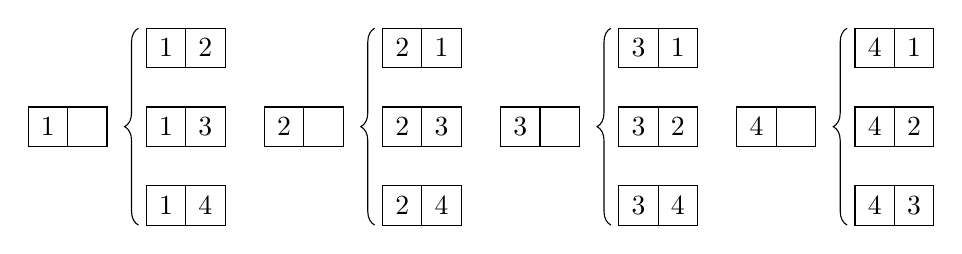
\begin{tikzpicture}
\begin{scope}
\draw(-.5,-.25) rectangle (.5,.25);
\draw(0,-.25)--(0,.25);
\node at (-0.25,0){1};
\foreach \x/\y in {-1/4,0/3,1/2}
{
    \draw(1, \x-.25) rectangle (2, \x+.25);
    \draw(1.5,\x-.25)--(1.5,\x+.25);
    \node at (1.25,\x){1};
    \node at (1.75,\x){\y};
}
\draw[decorate, decoration={brace, amplitude=5}](.9,-1.25)--(.9,1.25);
\end{scope}
\begin{scope}[xshift=3cm]
    \draw(-.5,-.25) rectangle (.5,.25);
    \draw(0,-.25)--(0,.25);
    \node at (-0.25,0){2};
    \foreach \x/\y in {-1/4,0/3,1/1}
    {
        \draw(1, \x-.25) rectangle (2, \x+.25);
        \draw(1.5,\x-.25)--(1.5,\x+.25);
        \node at (1.25,\x){2};
        \node at (1.75,\x){\y};
    }
    \draw[decorate, decoration={brace, amplitude=5}](.9,-1.25)--(.9,1.25);
    \end{scope}
    \begin{scope}[xshift=6cm]
        \draw(-.5,-.25) rectangle (.5,.25);
        \draw(0,-.25)--(0,.25);
        \node at (-0.25,0){3};
        \foreach \x/\y in {-1/4,0/2,1/1}
        {
            \draw(1, \x-.25) rectangle (2, \x+.25);
            \draw(1.5,\x-.25)--(1.5,\x+.25);
            \node at (1.25,\x){3};
            \node at (1.75,\x){\y};
        }
        \draw[decorate, decoration={brace, amplitude=5}](.9,-1.25)--(.9,1.25);
        \end{scope}
\begin{scope}[xshift=9cm]
\draw(-.5,-.25) rectangle (.5,.25);
\draw(0,-.25)--(0,.25);
\node at (-0.25,0){4};
\foreach \x/\y in {-1/3,0/2,1/1}
{
    \draw(1, \x-.25) rectangle (2, \x+.25);
    \draw(1.5,\x-.25)--(1.5,\x+.25);
    \node at (1.25,\x){4};
    \node at (1.75,\x){\y};
}
\draw[decorate, decoration={brace, amplitude=5}](.9,-1.25)--(.9,1.25);
\end{scope}
\end{tikzpicture}
\end{center}




\begin{example}
$a,b,c,d$四个元素,每次取出三个元素的不同排列有多少种,并写出所有的排列.(在同一排列里,元素不能重复出现.)
\end{example}

\begin{solution}
要把取出的三个元素排成一列,要分三步完成. 第一步先在第一个位置上放一个元素,应该有四种不同的方法;第二步要在第二个位置上放一个元素,由于第一步的工作完成后剩下的是三个元素,从三个元素中选一个放在第二个位置上应有3种不同的方法;第三步要在第三个位置上放一个元素,由于前两步工作完成后只剩下两个元素,所以只有两种不同的方法. 三步工作都完成后才完成排列工作,因此应该用乘法原理计算排列的总数,所以共有:$4\x4\x3\x2=24$种不同的排列.即有如下的24种不同的排列:
\begin{center}
\begin{tabular}{cccccc}
$abc$& $abd$& $acb$ &$acd$ &$adb$& $adc$\\
$bac$& $bad$ &$bca$& $bcd$ &$bda$& $bdc$\\
$cab$& $cad$ &$cba$& $cbd$ &$cda$& $cdb$\\
$dab$& $dac$& $dba$ &$dbc$& $dca$ &$dcb$    
\end{tabular}
\end{center}
\end{solution}

一般地说,从$n$个不同元素中,任取$m$个$(m\le n)$元素(不许重复),按照一定顺序排成一列的个数,叫做从$n$个不同元素中取出$m$个元素的排列数,用符号表示$\perm{m}{n}$.

\begin{blk}
  {定理1} 从$n$个不同元素中,任取$m$个$(m\le n)$没有重复的元素的排列数为$\perm{m}{n}=n(n-1)\cdots (n-m+1)$
\end{blk}

\begin{proof}
    在取出$m$个元素排成一列时,首先在第一个位置上可以选$n$个元素中的任何一个,故有$n$种方法. 在第二个位置上可以选余下的$n-1$个元素中的任一个.如此类推,在第$m$个位置上可以选余下的$(m-1)$个元素中的任一个. 根据乘法原理得到总的不同排列数应该是
\[\perm{m}{n}=m(n-1)\cdots(m-m+1)\]

这里的$m$是自然数,并且$m\le n$, 这个公式就叫做排列数公式.
\end{proof}

特别是当$m=n$时 有
\[\perm{n}{n}=n(n-1)\cdots3\cdot2\cdot1\]
这表示,$n$个不同的元素全部取出参加排列的排列数,叫做$n$个不同元素的全排列,自然数1到$n$的连乘积叫做$n$的阶乘,用$n!$表示,所以全排列数公式又可以写成
\[\perm{n}{n}=n!\]
有了阶乘,排列数公式又可以写成
\[\perm{m}{n}=\frac{n!}{(n-m)!}\]
这里,当$m=n$时,分母出现$(n-m)!$就变成$0!$,为了使公式仍能成立,我们特别规定$0!=1$.

例如$\perm{5}{8}=8\cdot  7\cdot 6\cdot 5\cdot 4=6720$,
$\perm{5}{5}=5!=5\cdot 4\cdot 3\cdot 2\cdot 1=120$

\begin{example}
    试证明下列等式成立.
\begin{multicols}{2}
\begin{enumerate}[(1)]
    \item $\perm{m}{n}+m\cdot \perm{m-1}{n}=\perm{m}{n+1}\quad (m\le n)$
\item $\perm{n+1}{n+1}-\perm{n}{n}=n^2\cdot \perm{n-1}{n-1}$
\end{enumerate}
\end{multicols}
\end{example}

\begin{proof}
\begin{enumerate}[(1)]
    \item \[\begin{split}
        \perm{m}{n}+m\cdot \perm{m-1}{n}&=\frac{n!}{(n-m)!}+m\cdot\frac{n!}{(n-m+1)!}\\
        &=\frac{(n-m+1)\cdot n!+m\cdot n!}{(n-m+1)!}=\frac{(n+1)\cdot n!}{(n-m+1)!}\\
        &=\frac{(n+1)!}{[(n+1)-m]!}=\perm{m}{n+1}
    \end{split}\]
所以原等式成立.

\item \[\begin{split}
    \perm{n+1}{n+1}-\perm{n}{n}&=(n+1)!-n!=(n+1)\cdot n!-n!\\
    &=n\cdot n!=n^2\cdot (n-1)!\\
    &=n^2\cdot \perm{n-1}{n-1}
\end{split}\]
所以原等式成立.
\end{enumerate}
\end{proof}

\begin{example}
    用0到9十个数字,可以写出多少个没有重复数的三位数?其中有多少个是偶数?
\end{example}

\begin{solution}
\begin{enumerate}[(1)]
    \item 第一步,因为0不能放在百位的位置上,所百位上的数有9种不同的选法,
    
第二步是从余下的九个数字中任选两个数字放在十位个位上,这有$\perm{2}{9}$种方法.所以
\[9\cdot \perm{2}{9}=9\cdot 9\cdot 8=648\]
\item 要得到三位偶数,必须个位上的数是0, 2, 6或8.但是0又不能排在百位上,这说明0怎样放在适合的置上是比其他问题要求更高的. 所以我们还是把0元素的题先解决.

第一类,0放在个位上这一选法确定后,其余百位、十位可以从余下的九个数字中任选两个数字放上去,这有$\perm{2}{9}$种方法.

第二类,个位上可放2,4,6,8中的任一个,在这类方法中,第一步在个位上有4种选法,第二步,在百位上可以放除0以外所余的八个字数的任一个,故有八种选择方法.第三步,余下的八个数字均可以放在十位上,所以
\[\perm{2}{9}+4\x8\x\perm{1}{8}=72+256=328\]
\end{enumerate}
答:有648个没有重复数字的三位数,其中有328个是偶数.

\end{solution}

关于例2.4中的第一个问题,我们还可以有如下的解法:

从0到9十个数字中任选三个数字排列总数为$\perm{3}{10}$.但是其中0在百位上的数有$\perm{2}{9}$个. 所以
\[\perm{3}{10}-\perm{2}{9}=10\cdot 9\cdot 8-9\cdot 8=648\]

\begin{ex}
\begin{enumerate}
    \item 写出从$a,b,c,d,e$中任取两个不同元素的所有排列.
    \item 计算:
\begin{multicols}{3}
\begin{enumerate}[(1)]
    \item $\perm{3}{7}$
    \item $\perm{3}{15}$
    \item $\perm{4}{4}$
    \item $\perm{4}{8}-3\cdot\perm{2}{8}$
    \item $\perm{3}{7}-5\perm{2}{7}$
    \item $\frac{\perm{7}{12}}{\perm{6}{11}}$
\end{enumerate}
\end{multicols}

\item 求证:
\begin{enumerate}[(1)]
    \item $n!=\frac{(n+1)!}{n+1}$
    \item $\perm{m}{n}=\frac{\perm{n+2}{n+2}}{\perm{2}{n+2}\cdot \perm{n-m}{n-m}}\quad (m\le n)$
\end{enumerate}

\item 某一段铁路共有8个车站,需要为这段铁路印制多少种不不同的客车票?(都是普通座位票)
\item 6个同学排成一列,有多少种不同的排法?
\item 从12人的1个学习小组中,选1个正组长和1个副组长,问有多少种不同的选法?
\item 用0至5共六个数字,可以组成多少不同的三位数?
\item 用0到9这十个数字,其中有多少个没有重复数字的二位数,其中有多少个二位奇数?
\item 某信号兵用红、黄、篮三面旗子从上到下挂在竖直的旗杆上表示信号,每次可以任挂一面、二面或三面,并且不同的顺序表示不同的信号,问一共可以表示多少种不同的信号?
\item 有五道不同的工序分配给五个工人工作,其中有一个工人不会做其中两道工序,问有多少种不同的分配法?
\item 由2, 3, 4, 5所组成的没有重复数字的四位数,
\begin{enumerate}[(1)]
\item 求所有这些四位数里各个数字的和;
\item 求所有这些四位数的和。
\end{enumerate}
\end{enumerate}
\end{ex}

\section{组合}
我们知道,从一个学习小组中选出正、副组长各1人,这种选法是排列问题.如果改变为从一个学习小组中选出代表2人参加学校的学代会,有多少种不同的选法?”这时的代表无所谓正、副之分,就无先后顺序的意义了,也就不成为排列的问题了.

又例如从1, 2, 3, 4, 5五个数选出两个数字相乘,问有多少个不同的乘积?那么只要所选出的数字是3和5;它们的积只有15,至于是$5\x3$还有$3\x5$,那是不要求加以区别的,也是没有排列次序的区别的.

一般地说,从$n$个不同的元素中,任取$m\; (m\le n)$个元素并成一组,叫做从$n$个不同元素中取出$m$个元素的一个组合.

这里要注意,元素$a$,$b$,$c$的组合与$a,c,b$; $c,a,b$; $b,a,c$; $b,c,a$或$c,b,a$都被看作是相同的组合了. 对于排列来说,上列的是六个不同的排列,而对于组合来说,只算是一个组合,那么组合数是怎样进行计算的呢?

从$n$个不同元素中取出$m\; (m\le n)$个元素的所有组合的个数,叫做从$n$个不同元素中取出$m$个元素的组合数,用符号$\comb{m}{n}$表示。

例如,从四个不同元素中取出3个元素进行排列,有多少种不同的排法?

我们已经知道应该有$\perm{3}{4}=24$种不同的排法,现在我们
想从另外的方法入手解决这个问题.

第一步,从$a,b,c,d$中取三个元素作一组,这样可以得到$a,b,c$; $a,b,d$; $a,c,d$; $b,c,d$四个组,这就是说$\comb{3}{4}=4$.

第二步,把每组的三个元素作全排列,应有$\perm{3}{3}$个不同排列.

根据乘法原理得$\perm{3}{4}=4\cdot \perm{3}{3}$,即$\perm{3}{4}=\comb{3}{4}\cdot \perm{3}{3}$.

又如,从五个不同的元素中取出2个元素的列排数是$\perm{2}{5}$. 如果我们从五个不同元素中取出两个分成一组,我们可以组成如下的小组:

$a,b$; $a,c$; $a,d$; $a,e$; $b,c$; $b,d$; $b,e$; $c,d$, $c,e$和$d,e$等10个组,这就是$\comb{2}{5}$;第二步把每组元素进行全排列应是$\perm{2}{2}$,这样应该有$\perm{2}{5}=\comb{2}{5}\cdot \perm{2}{2}$. 因此,一般地说,从$n$个不同元素中取出$m\; (m\le n)$个元素的排列数$\perm{m}{n}$可以等于$\comb{m}{n}\cdot \perm{m}{m}$.


\begin{blk}
  {定理2} 从$n$个不同元素中任取$m$个($m\le n$)没有重复元素组合数为$\comb{m}{n}=\frac{n!}{m!(n-m)!}$.  
\end{blk}

\begin{proof}
    由$\perm{m}{n}=\comb{m}{n}\cdot \perm{m}{m}$,所以
\[\comb{m}{n}=\frac{\perm{m}{n}}{\perm{m}{m}}=\frac{\frac{n!}{(n-m)!}}{m!}=\frac{n!}{m!(n-m)!}\]
\end{proof}
注意:$\comb{m}{n}=\frac{n(n-1)\cdots(n-m+1)}{m!}$

\begin{example}
计算$\comb{3}{8}$, $\comb{5}{8}$和$\comb{2}{9}$
\end{example}

\begin{solution}
    根据组合数公式有:
\[\begin{split}
    \comb{3}{8}&=\frac{8\x 7\x 6}{3\x 2\x 1}=56\\
    \comb{5}{8}&=\frac{8\x 7\x 6\x 5\x 4}{5\x 4\x 3\x 2\x 1}=56\\
    \comb{2}{9}&=\frac{9\x 8}{2\x 1}=36
\end{split}\]
\end{solution}

组合数有以下性质:
\begin{blk}
{性质1}$$\comb{m}{n}=\comb{n-m}{n}$$
\end{blk}

\begin{proof}
根据组合数公式:
\[\begin{split}
    \comb{m}{n}&=\frac{n!}{m!(n-m)!}\\
    \comb{n-m}{n}&=\frac{n!}{(n-m)![n-(n-m)]!}=\frac{n!}{m!(n-m)!}
\end{split}\]
所以$\comb{m}{n}=\comb{n-m}{n}$.
\end{proof}

\begin{blk}{性质2}
\[\comb{m}{n+1}=\comb{m}{n}+\comb{m-1}{n}\]
\end{blk}

\begin{proof}
根据组合数公式:
\[\begin{split}
    \comb{m}{n+1}&=\frac{(n+1)!}{m!(n-m+1)!}\\
    \comb{m}{n}+\comb{m-1}{n}&=\frac{n!}{m!(n-m)!}+\frac{n!}{(m-1)!(n-m+1)!}\\
    &=\frac{(n-m+1)\cdot n! +m\cdot n!}{m!(n-m+1)!}=\frac{n!\cdot (n-m+1+m)}{m!(n-m+1)!}\\
    &=\frac{(n+1)!}{m!(n-m+1)!}\\
\end{split}\]
所以$\comb{m}{n+1}=\comb{m}{n}+\comb{m-1}{n}$.
\end{proof}

为了使性质1在$n=m$时也能成立,我们规定$\comb{0}{n}=1$.

\begin{example}
计算$\comb{98}{100}$和$\comb{2}{10}+\comb{3}{10}+\comb{2}{11}+\comb{2}{12}$
\end{example}

\begin{solution}
根据组合数性质1
\[\comb{98}{100}=\comb{100-98}{100}=\comb{2}{100}=\frac{100\x 99}{2\x 1}=4950\]
根据组合数性质2
\[\begin{split}
    \comb{2}{10}+\comb{3}{10}+\comb{2}{11}+\comb{2}{12}&=\comb{3}{11}+\comb{2}{11}+\comb{2}{12}\\
    &=\comb{3}{12}+\comb{2}{12}=\comb{3}{13}\\
    &=\frac{13\x 12\x 11}{3\x 2\x 1}=286
\end{split}\]
\end{solution}

\begin{example}
    解不等式 $\comb{3}{n}>\comb{5}{n}$
\end{example}

\begin{solution}
\[\frac{n(n-1)(n-2)}{3\x 2\x 1}>\frac{n(n-1)(n-2)(n-3)(n-4)}{5\x 4\x 3\x 2\x 1}\]
因为$5\le n$,所以$n,\; n-1,\; n-2,\; n-3,\; n-4$均为正数,所以
\[1>\frac{(n-3)(n-4)}{5\x 4}\]
整理得:$n^2-7n-8<0$

解不等式得:$-1<n<8$,根据题意,得:$n=5,6,7$.
\end{solution}



\begin{example}
高中三个年级,每个年级有六个班。
\begin{enumerate}[(1)]
\item 每级都进行单循环(每班都与级内其他各班比赛一场)篮球预赛,问预赛需要比赛多少场?
\item 从各级预赛中选出每级的冠、亚军,再进行单循环决赛,规定在预赛中已经比赛过的队不再比赛,问决赛需要比赛多少场?
\end{enumerate}
\end{example}

\begin{solution}
\begin{enumerate}[(1)]
    \item 根据题意每个级单循环比赛的场次都是$\comb{2}{6}$,所以
\[3\comb{2}{6}=3\times 15=45\]
\item 决赛共6个班,如果单循环要比赛$\comb{2}{6}$场,但预赛中比赛过的有3场,所以
\[\comb{2}{6}-3=15-3=12\]
\end{enumerate}
答:预赛要比赛45场,决赛要比赛12场.
\end{solution}



\begin{example}
    平面有10个不同的点,其中除4个点在同一直线上外,不再有3个点共线,以每三个点为顶点可以作多少个不同的三角形?
\end{example}


\begin{solution}
    如果10点中的任三点都能连成三角形,那么有$\comb{3}{10}$个三角形. 但是如果在四个共线点中任选三点就不可能构成三角形. 所以
\[\comb{3}{10}-\comb{3}{4}=120-4=116\]
答:可以作116个不同的三角形。
\end{solution}



\begin{example}
    在产品检验时,常从产品中抽出一部分进行检查,假设100件产品中有2件次品,
    \begin{enumerate}[(1)]
        \item 从100件产品中抽出三件检查,其中有1件次品的抽法有多少种?
        \item 从100件产品中抽出4件检查,其中至少有一件次品的抽法有多少种?
    \end{enumerate}
\end{example}

\begin{solution}
\begin{enumerate}[(1)]
    \item 在100件产品中,次品有两件,从2件次品中抽出1件的抽法有$\comb{1}{2}$,从98件正品中抽出2件的方法有$\comb{2}{98}$. 所以
\[\comb{1}{2}\cdot \comb{2}{98}=2\cdot \frac{98\cdot 97}{2}=9506\]
    \item 至少有1件是次品就是包括有1件次品和2件次品两类抽法的和,所以 
\[\comb{1}{2}\cdot \comb{3}{98}+\comb{2}{2}\cdot \comb{2}{98}=2\times \frac{98\cdot 97\cdot 96}{3\cdot 2}+\frac{98\cdot 97}{2}=304192+4753=308945\]
\end{enumerate}
答:3件中有1件是次品的抽法是9506, 4件中至少有1件次品的抽法是308945。
\end{solution}

\begin{example}
    从0, 3, 5, 7, 11五个数中可以得到多少个不同的乘积?
\end{example}

\begin{solution}
    因为零乘以任何数其积都是零,所以不论零与多少个数相乘都只算一个乘积就是0;

在非零的乘积中有$\comb{2}{4}$, $\comb{3}{4}$, $\comb{4}{4}$三类,所以
\[\comb{2}{4}+\comb{3}{4}+\comb{4}{4}+1=6+4+1+1=12\]

答:可以得到12个不同的乘积.
\end{solution}

\begin{ex}
\begin{enumerate}
    \item 写出:
    \begin{enumerate}[(1)]
    \item 从4个相异元素$a$,$b$,$c$,$d$中取出2个元素的所有组合;
    \item 从5个相异元素$a$,$b$,$c$,$d$,$e$中取出3个元素的所有组合.
    \end{enumerate}

    \item 计算:
\begin{multicols}{2}
\begin{enumerate}[(1)]
    \item  $\comb{2}{7}$
    \item $\comb{48}{50}$
    \item $\comb{3}{100}-\comb{3}{90}$
    \item $\comb{1}{5}+\comb{2}{5}+\comb{3}{5}+\comb{4}{5}+\comb{5}{5}$
\end{enumerate}
\end{multicols}
    
\item   平面内有12个点,其中任意3点不在同一直线上,以每3点为顶点作一三角形,一共可以作多少个不同的三角形?
\item 圆上$n$个不同的点,
\begin{enumerate}[(1)]
\item 可以引多少条不同的弦?
\item 可以连接多少个内接三角形?
\end{enumerate}

\item 凸四边形可以连多少条对角线?凸五边形可以连多少条对角线?凸$n$边形可以连多少条对角线?
\item 某班有50名学生,其中正副班长各1人,现选5名学生参加某项活动
\begin{enumerate}[(1)]
\item 如果班长和副班长必须在内,有多少种不同的选法?
\item 如果要有一个班长(正、副都可以)在内,有多少种不同的选法?
\item 如果班长都不参加,有多少种不同的选法?
\item 如果至少要有一个班长(正、副都可以)在内,有多少种不同的选法?
\end{enumerate}
\end{enumerate}
\end{ex}

\section*{习题2.1}
\begin{enumerate}
    \item 计算:
\begin{multicols}{2}
\begin{enumerate}[(1)]
    \item $5\cdot \perm{3}{5}+4\cdot \perm{2}{4}$
    \item $\frac{\perm{5}{7}-\perm{6}{6}}{7!+6!}$
\end{enumerate}
\end{multicols}

\item 求证:
\begin{enumerate}[(1)]
    \item $\frac{(n+1)!}{k!}-\frac{n!}{(k-1)!}=\frac{(n-k+1)\cdot n!}{k!}$
    \item $\frac{(2n)!}{2^n \cdot n!}=1\cdot 3\cdot 5\cdots (2n-1)$
\end{enumerate}

\item 解方程:
\begin{multicols}{2}
\begin{enumerate}[(1)]
    \item $\perm{3}{2n}=10\perm{3}{n}$
    \item $\frac{\perm{5}{n}+\perm{4}{n}}{\perm{3}{n}}=4$
    \item $\perm{4}{2n+1}=140\perm{3}{n}$
\end{enumerate}
\end{multicols}

\item 解不等式:
\begin{multicols}{2}
\begin{enumerate}[(1)]
    \item $\perm{2}{m-2}+m>2$
    \item $\perm{x}{9}>6\perm{x-2}{9}$
\end{enumerate}
\end{multicols}

\item \begin{enumerate}[(1)]
    \item 从多少个不同的元素中取出2个元素的排列数是56?
    \item 已知从$n$个不同的元素中取出2个元素的排列数等于从$n-4$个不同元素中取2个元素的排列数的7倍,求$n$.
\end{enumerate}
\item 有5本不同的书分借给3个同学,每人1本,共有多少种不同的借法?
\item 用0, 1, 2, 3, 4, 5可以组成多少个没有重复数字的五位数?其中有多少个偶数?
\item 用数字1, 2, 3, 4, 5可以组成多少个没有重复数字的自然数?其中有多少个比13000大的自然数?
\item 7部不同型号的机床分配给7个工人使用:
\begin{enumerate}[(1)]
\item 甲必须使用2号机床;
\item 甲必须使用2号机床,乙必须使用4号机床;
\item 甲不适宜使用1号机床,乙不适宜使用7号机床;问三种情况下各有多少种不同的分配方案?
\end{enumerate}

\item 6个儿童站成一排,其中一人不站在排头,也不站在排尾,一共有多少种不同的排法?
\item 五部不同型号的半导体收音机和四部不同型号的电视机陈列成一排,任两部电视机不靠在一起,有多少种不同的陈列方法?
\item 在3000和7000间有多少个没有重复数字的5的倍数?

\item 计算:
\begin{multicols}{2}
\begin{enumerate}[(1)]
    \item $\comb{3}{15}$
    \item $\comb{98}{100}$
    \item $\comb{3}{6}+\comb{6}{8}$
    \item $\comb{n}{n+1}\cdot \comb{n-2}{n}$
\end{enumerate}
\end{multicols}

\item 求证:
\begin{enumerate}[(1)]
    \item $\comb{m}{n+1}=\comb{m-1}{n}+\comb{m}{n-1}+\comb{m-1}{n-1}$
    \item $\comb{k+1}{n}\div \comb{k}{n}=\frac{n-k}{k+1}$
    \item $\comb{0}{m}+\comb{1}{m+1}+\comb{2}{m+2}+\cdots+\comb{n-1}{m+n-1}=\comb{n-1}{m+n}$
    \item $\comb{m+1}{n}+\comb{m-1}{n}+2\comb{m}{n}=\comb{m+1}{n+2}$
\end{enumerate}

\item 解不等式:
\begin{multicols}{2}
\begin{enumerate}[(1)]
    \item $\comb{n}{4}>\comb{n}{6}$
    \item $\comb{n-4}{21}<\comb{n-2}{21}<\comb{n-1}{21}$
\end{enumerate}
\end{multicols}

\item 在200件产品中有2件次品,现在抽5件进行检查:
\begin{enumerate}[(1)]
\item 其中有一件次品的不同抽法有多少种?
\item 没有次品的不同抽法有多少种?
\item 至少有一件次品的不同抽法有多少种?
\end{enumerate}

\item 问2310能被多少个偶数整除?
\item 有8个划船运动员,其中3人能划左舷,2人能划右舷,3人能划左右舷,要选出6人分配在两边,问有多少种不同的选法?

\item  某车间有9名技术熟练的工人,其中2人能当车、钳工,有3人只能当车工,其余4人只能当钳工,现在要抽调三个车工,三个钳工成立一个新车间,问有多少种不同的抽调方法?
\item  空间有12个不同的点,其中有4点在同一平面内,此外不再有4点共面,
\begin{enumerate}[(1)]
\item  这些点可以确定多少个不同的平面?
\item  这些点可以连成多少个不同的四面体?
\end{enumerate}

\item  有8部机器分给陈、李、张三位师傅管理。
\begin{enumerate}[(1)]
\item 陈管4部,李管3部,张管1部,有几种不同分配方法?
\item 陈管4部,其他机器由1人管3部,1人管1部,有多少种不同的分配方法?
\item 1人管4部,一人管3部,一人管1部,有几种不同的分配方法?
\end{enumerate}

\item  从1, 5, 7, 9中任取3个数字,2, 4, 6, 8中任取两个数字,组成没有重复数字的五位数,一共有多少个不同的五位数?
\end{enumerate}

\section{环形排列、重复排列和组合}
\subsection{环形排列}
我们已经学握了从$n$个相异的元素中取出$m\; (m\le n)$个元素的排列的知识了,那么怎样解决环形排列的问题呢?

我们先从最简单的情况入手,就是先找出环形排列与直
线排列的相互关系,然后利用直线排列的知识解决环形排列的问题.

首先在环形排列中,下面的排列都是当作相同的排列的(图2.2).
\begin{figure}[htp]
    \centering
\begin{tikzpicture}[>=stealth]
\begin{scope}
\draw circle(.9);
\node at (90:1.2){甲};
\node at (90+180:1.2){乙};
\draw[->](90-20:1.2) arc (90-20:20:1.2);
\end{scope}
\begin{scope}[xshift=3cm]
\draw circle(.9);
\node at (0:1.2){甲};
\node at (0+180:1.2){乙};
\draw[->](0-20:1.2) arc (0-20:-70:1.2);
\end{scope}
\begin{scope}[xshift=6cm]
\draw circle(.9);
\node at (-90:1.2){甲};
\node at (-90+180:1.2){乙};
\draw[->](-90-20:1.2) arc (-90-20:-160:1.2);
\end{scope}
\begin{scope}[xshift=9cm]
\draw circle(.9);
\node at (45:1.2){甲};
\node at (45+180:1.2){乙};
\draw[->](45-20:1.2) arc (45-20:-20:1.2);
\end{scope}

\end{tikzpicture}
    \caption{}
\end{figure}


因为从甲开始,按同一方向,例如顺时针方向看过去都是乙,所以尽管位置不同,但仍然是同一样的元素的排列顺序.
\begin{figure}[htp]
    \centering
\begin{tikzpicture}[>=stealth]
\begin{scope}
\draw circle(.9);
\node at (90:1.2){甲};
\node at (90-120:1.2){乙};
\node at (90+120:1.2){丙};
\draw[->](90-20:1.2) arc (90-20:20:1.2);
\end{scope}
\begin{scope}[xshift=3.5cm]
\draw circle(.9);
\node at (0:1.2){甲};
\node at (0-120:1.2){乙};
\node at (0+120:1.2){丙};
\draw[->](0-20:1.2) arc (0-20:-70:1.2);
\end{scope}
\begin{scope}[xshift=7cm]
\draw circle(.9);
\node at (-90:1.2){甲};
\node at (-90-120:1.2){乙};
\node at (-90+120:1.2){丙};
\draw[->](-90-20:1.2) arc (-90-20:-160:1.2);
\end{scope}
  
\end{tikzpicture}
    \caption{}
\end{figure}


又例如三个不同元素甲、乙、丙如图2.3的三个环形排列也都算是相同的排列,而且与从谁开始无关,即甲$\to $乙$\to $丙$\to $甲、乙$\to $丙$\to $甲$\to $乙与丙$\to $甲$\to $乙$\to $丙,也都算作是相同的环形排列.

从上述的例子,可以得到三个不同元素的环形排列数应该是2.具体的排列是:甲—乙—丙—甲与甲—丙—乙—甲.

现在,我们再来分析一下环形排列与直线排列不同的特点. 我们已经知道下列三个环形排列都是相同的排列(图2.4)
\begin{figure}[htp]
    \centering
\begin{tikzpicture}[>=stealth]
\begin{scope}
\draw circle(.9);
\node at (90:1.2){甲};
\node at (90-120:1.2){乙};
\node at (90+120:1.2){丙};
\draw[->](-.35,1.5)--(-.35,1);
\end{scope}
\begin{scope}[xshift=3.5cm]
    \draw circle(.9);
    \node at (90:1.2){丙};
    \node at (90-120:1.2){甲};
    \node at (90+120:1.2){乙};
    \draw[->](-.35,1.5)--(-.35,1);

    \end{scope}
\begin{scope}[xshift=7cm]
    \draw circle(.9);
    \node at (90:1.2){乙};
    \node at (90-120:1.2){丙};
    \node at (90+120:1.2){甲};
    \draw[->](-.35,1.5)--(-.35,1);

    \end{scope}
\end{tikzpicture}
    \caption{}
\end{figure}

如果我们从图上所示的地方把环切断,并把环拉成直线后,我们却可以得到三个不同的直线的排列,就是:
\[\text{甲、乙、丙;丙、甲、乙;乙、丙、甲}\]

而三个不同元素的全排列数是$\perm{3}{3}$,所以三个不同元素的环形排列数是$\frac{\perm{3}{3}}{3}$

\begin{blk}
    {定理3} $m$个不同元素的环形排列数就是:
\[\frac{\perm{m}{m}}{m}=\frac{m!}{m}=(m-1)!\]
\end{blk}

\begin{proof}
    
\end{proof}
设有$m$个不同元素排成一个环形,如图(图2.5)
\begin{figure}[htp]
    \centering
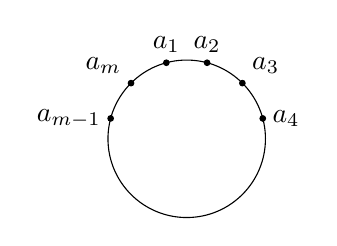
\begin{tikzpicture}
\draw(0,0) circle(1);
\draw[fill](15:1)node[right]{$a_4$} circle(1pt);
\draw[fill](15+30:1)node[above right]{$a_3$} circle(1pt);
\draw[fill](15+60:1)node[above]{$a_2$} circle(1pt);
\draw[fill](15+90:1)node[above]{$a_1$} circle(1pt);
\draw[fill](15+120:1)node[above left]{$a_m$} circle(1pt);
\draw[fill](15+150:1)node[left]{$a_{m-1}$} circle(1pt);
\end{tikzpicture}
    \caption{}
\end{figure}
就是按顺时针方向的一个排列.其次,$a_1$不动,改变$a_2,a_3,\ldots,a_m$的顺时针排列顺序,就得到第二个不同的环形排列.因此,如果$a_1$不动,要使$a_2,a_3,\ldots,a_m$有不同的排
列,其不同的排列数为$(m-1)!$,故$m$个不同元素的环形排列数为$\perm{m-1}{m-1}=(m-1)!$


\begin{blk}
  {定理4} 从$n$个不同的元素中,任取$m$个($m\le n$)没有重复的元素的环形排列数$\comb{m}{n}\cdot (m-1)!$.  
\end{blk}

\begin{proof}
    从$n$个不同元素中取出$m\; (m\le n)$个元素进行环形排列,我们第一步可以先从$n$个元素中先取出$m$个组成一组,第二步是把$m$个元素排成一圈,根据乘法原理,其排列数应为:
\[\comb{m}{n}\cdot \perm{m-1}{m-1}=\comb{m}{n}(m-1)!\]
\end{proof}

\begin{example}
    从10个不同元素中取出6个元素排成一圈,有多少种不同的排法?
\end{example}

\begin{solution}
    从10个不同元素中取出6个的环形排列数为:
\[\comb{6}{10}\cdot\perm{6-1}{6-1}=\comb{4}{10}\cdot  5!=210\cdot 120=25200\]
答:有25200种不同的排法.
\end{solution}

\begin{example}
    有五个男同学与五个女同学围成圆圈跳集体舞,如果男女相间,问有几种不同的排列方法?
\end{example}

\begin{solution}
第一步,五个男同学先作环形排列,其排列数为$4!$;

第二步,五个女同学分别站在两个男同学之间的位置上作全排列.

$\therefore\quad 4! \cdot 5! =2880$

答:有2880种不同的排列方法.    
\end{solution}

\begin{ex}
\begin{enumerate}
\item 把10个人平均分成两组,每组都围坐一个圆桌,问有多少种不同的坐法?
\item 今有5颗不同颜色的珠子,用线把它们串成珠圈,间有多少种串法?
\end{enumerate}
\end{ex}

\subsection{重复排列}

前面我们所研究的都是不允许元素在排列和组合中重复出现的,假如我们允许元素在同一排列中重复出现的话,其排列数应该是多少呢?

\begin{blk}
{定理5} 从$n$个不同的元素中,取出$m$个元素排成一列(允许元素重复出现)的不同排列数为$n^m$.
\end{blk}

\begin{proof}
    选在第一个位置上的元素有$n$个不同的方法,选在第二个位置上的元素仍然有$n$个不同的方法,……,选在第$m$个位置上的元素仍然有$n$个选法,所以根据乘法原理,从$n$个不同的元素中取出$m$个元素的允许重复的排列数应为$n^m$.
\end{proof}

这种排列又称为重复排列,这里应该注意的是,由于元素可以重复选取,因此选取的次数$m$就不会再受$n$个元素的限制. 即$m$不再有$m\le n$的限制了.

\begin{example}
    电报通讯的明码是用0到9十个数字中的每4个数字的重复排列代表一个汉字,问用这种方法制成的电报通讯明码可以表示多少个不同的汉字?
\end{example}

\begin{solution}
    从10个不同数字中选取4个数字的重复排列数是:
\[10^4=10000\]
答:可以表示10000个不同的汉字.
\end{solution}

\begin{example}
    由1, 2, 3, 4四个数字能够组成多少个大于2300的四位数?
\end{example}

\begin{solution}
    这里的四位数显然是包括重复数字的四位数.

第一类:3在千位上的四位数一定大于2300,那么,百、十、个位上的数字每次都有4种选取可能,所以应有$4^3$个四位数.

第二类:4在千位上的四位数,同理也有$4^3$个四位数。

第三类:2在千位上,3在百位上的四位数,由于十位和个位上的数都可以从1, 2, 3, 4中选取,都大于2300,所以,这样的数有$4^2$个.

第四类,2在千位上,4在百位上的四位数有$4^2$个.所以
\[2\cdot 4^3+2\cdot 4^2=2\cdot 4^2(4+1)=160\]

答:这样的四位数有160个.
\end{solution}

\begin{ex}
    \begin{enumerate}
\item 有三封不同的信,投入4个信箱里,一共有多少种投信的方法?
\item 有数学、天文、诗歌三个课外小组,8个同学准备报名,若每人限报一个组,问一共可有多少种报名的方法?
    \end{enumerate}
\end{ex}

\subsection{重复组合}
从$n$个不同元素中取出$m$个元素组成一组,如果允许元素在组合中重复出现,这样的组合简称为重复组合,这种重复组合用符号$\rep{m}{n}$表示.

怎样计算重复组合的组合数呢?我们还是先从具体例子开始考虑,假如有三个不同的元素$a_1,a_2,a_3$,从其中取出两个元素组成重复组合,那么,可以得到如下的六个不同组合:
\begin{equation}
a_1a_1,\; a_1a_2,\; a_1a_3,\; a_2a_1,\; a_2a_3,\; a_3a_3 \tag{1}
\end{equation}

如果是不允许元素重复的话,要选两个元素得到不同的组合数是6的话,应是$\comb{2}{4}$,设这四个元素为$a'_1,a'_2,a'_3,a'_4$,那么得到的组合为:
\begin{equation}
a'_1a'_2,\; a'_1a'_3,\; a'_1a'_4,\; a'_2a'_3,\; a'_2a'_4,\; a'_3a'_4 \tag{2}
\end{equation}
组合(1)与组合(2)不难建立它们之间的一一对应关系.在组合(1)的每个组合的元素下标上分别加上0和1,就得到了下标与(2)完全一致的组合(3).
\begin{equation}
a_{1+0}a_{1+1},\quad a_{1+0}a_{2+1},\quad a_{1+0}a_{3+1},\quad a_{2+0}a_{2+1},\quad a_{2+0}a_{3+1},\quad a_{3+0}a_{3+1}
\tag{3}
\end{equation}

又例如从4个不同元素中取出3个元素的重复组合有如下的不同组合:
\begin{center}
\begin{tabular}{ccccc}
    $a_{1}a_{1}a_{1}$&$a_{1}a_{1}a_{2}$&$a_{1}a_1a_{3}$&$a_{1}a_{1}a_{4}$\\
    &$a_{1}a_{2}a_{2}$&$a_{1}a_{2}a_{3}$&$a_{1}a_{2}a_{4}$\\
    &$a_{1}a_{3}a_{3}$&$a_{1}a_{3}a_{4}$&$a_{1}a_{4}a_{4}$\\
    &$a_{2}a_{2}a_{2}$&$a_{2}a_{3}a_{3}$&$a_{2}a_{2}a_{4}$\\
    &$a_{2}a_{3}a_{3}$&$a_{2}a_{3}a_{4}$&$a_{2}a_{4}a_{4}$\\
 &$a_{3}a_{3}a_{3}$&$a_{3}a_{3}a_{4}$&$a_{3}a_{4}a_{4}$\\
   &$a_{3}a_{3}a_{3}$&$a_{3}a_{3}a_{4}$&$a_{3}a_{4}a_{4}$&$a_{4}a_{4}a_{4}$\\ 
\end{tabular}
\end{center}

只要我们在每组元素的下标上分别加0, 1, 2, 就得到
\begin{center}
\begin{tabular}{ccccc}
    $a_{1}a_{2}a_{3}$&$a_{1}a_{2}a_{4}$&$a_{1}a_{2}a_{5}$&$a_{1}a_{2}a_{6}$\\
 & $a_{1}a_{3}a_{4}$&$a_{1}a_{3}a_{5}$&$a_{1}a_{3}a_{6}$\\
 &$a_{1}a_{4}a_{5}$&$a_{1}a_{4}a_{6}$&$a_{1}a_{5}a_{6}$\\
 &$a_{2}a_{3}a_{4}$&$a_{2}a_{3}a_{5}$&$a_{2}a_{3}a_{6}$\\
 &$a_{2}a_{4}a_{5}$&$a_{2}a_{4}a_{6}$&$a_{2}a_{5}a_{6}$\\
 &$a_{3}a_{4}a_{5}$&$a_{3}a_{4}a_{6}$&$a_{3}a_{5}a_{6}$&$a_{4}a_{5}a_{6}$
\end{tabular}
\end{center}

这又正是从六个不同元素中取出3个元素的组合的全部。
从上面的例子说明了
\[{\rm H}_{3}^{2}= {\rm C}_{3+ ( 2- 1) }^{2}, \qquad {\rm H}_{4}^{3}={\rm C}_{4+ ( 3- 1) }^3\]

按同样的方法我们可以得出:从$n$个不同元素中取出$m$
个的重复组合数有如下的关系:
$${\rm H}_{n}^{m}= {\rm C}^m_{n+ ( m- 1) }$$

现在我们来证明这个结论.

\begin{blk}
 {定理6} 从$n$个不同元素中,任取$m$个元素 的重复组合为:
 $${\rm H}_{n}^{m}={\rm C}_{n+ ( m-1) }^{m}$$ 
\end{blk}

\begin{proof}
    为了研究问题方便,我们用$1,2,3,\ldots,n$表示这$n$个不同的元素。在其中任取$m$个允许重复的数字作为一个组合,并按大小顺序排成
$$1\le  i_2\le i_2\le\cdots\le i_m\le n$$

    又记$j_1=i_1+0,\; j_{2}=i_{2}+1,\;\ldots, j_{m}=i_{m}+(m-1)$
    
    自然,$1\le j_1<j_2<j_3<\cdots<j_m\leq n+(m-1)$,所以$\{j_1,j_2,\ldots,j_m\}$ 是$n+ m- 1$个 数,并 且 是$1, 2, \ldots , n+m-1$中的$m$个不同数的组合.
\end{proof}

下面来证明:在$n$个不同元素中任取$m$个允许重复的元
素的组合,和$n+m-1$个不同元素中任取$m$个不同元素 的组合之间有一个到上的一一对应关系。如果这点证明了,那么$n$个不同元素的$m$个允许重复元素的组合数就与$n+m-1$个不同元素的$m$个不同元素的组合数相等了.

\begin{proof}
    
为了证明这个一一对应,要先证明当允许重复的组合
$\{i_1,i_2,\ldots,i_m\}$与$\{i_1^{\prime},i_2^{\prime},\ldots,i'_m\}$不同 的时候,
(这里取$1\le i_1\le i_2\le\cdots\le i_m\le n$, $1\le i'_1\le i'_2\le\cdots\le i^{\prime}_m\le n$)那么,不同元素不允许重复的组合$\{j_1,i_2,\ldots, i_m\}$与$\{j_1^{\prime},j_2^{\prime},\ldots,j'_m\}$也不同,这里$\{j_1=i_1+0,\; j_2=i_{2}+1,\ldots,j_{m}=i_{m}+m-1,\; j_{1}^{\prime}=i_{1}^{\prime}+0,\; j_{2}^{\prime}=i_{2}^{\prime}+1,\ldots, j_m^{\prime}=i_m^{\prime}+m-1\}$.

事实上,如果后者相同,即有$j_{k}= j_{k}\; (k= 1, 2, \ldots, m)$ 即
$$i_k+k-1=i_k^{\prime}+k-1\; (k=1,2,\ldots,m)$$ 
所以$i_k= i_k^{\prime }\; ( k= 1, 2, \ldots , m)$, 也就是说$\{i_1, i_2,\ldots,i_m\}$也与$\{i_1^{\prime},i_2^{\prime},\ldots,i_m^{\prime}\}$相同了。这就证明了上述的对应为一一对应.

再证明这是到上的一一对应,即当$\{i_1,i_2,\ldots,i_m\}$取遍$n$个数$1,2,\ldots,n$的一切$m$个数的允许重复组合时,$\{j_i, j_2,\ldots,j_m\}$ 也取遍$n+m-1$个 数 $1,2,\ldots ,n+m-1$一切的 $m$ 个数的不允许重复的组合.

事实上,对任一个组合$\{j_1,j_2,\ldots,j_m\}$, 其中$1\le j_{1}<j_{2}<\cdots<j_{m}\le n+m-1$. 有$1\leq j_{1},\; 2\le j_{2},\; 3\le j_{3},\ldots, m\le j_{m}$. 故$1\le i_1=j_1-0,\; 1\le i_2=j_2-1,\; 1\le i_3=j_3-2,\ldots, 1\leq i_m=j_m-(m-1)$. 即$i_1,i_2,\ldots,i_m$都是自然数,且由$j_{k}>j_{k-1}$, 可知$j_k-j_{k-1}\ge 1$, 故有
\[i_k-i_{k-1}=[j_k-(k-1)]-[j_{k-1}-(k-2)]=j_k-j_{k-1}-1\ge 0\]
再者$i_{m}=j_{m}-(m-1)\le (n+m-1)-(m-1)=n$. 总之有$1\le i_1\le i_2\le \cdots \le i_m\le n$. 所以,$\{i_1,i_2,\ldots,i_m\}$ 是$n$个数$1,2,\ldots,n$中取$m$个数的允许重复的组合,这证明了对应是到上的一一对应.

\end{proof}


\begin{example}
  从3, 5, 7, 9, 11中取出3个数(可以重复选取)相乘,问有多少个不同的乘积?  
\end{example}

\begin{solution}
    因为是乘积,与元素取出的先后顺序无关,同时是可以重复选取的,即是重复组合问题. 所以
\[{\rm H}^3_5=\comb{3}{5+(3-1)}=\comb{3}{7}=35\]
答:有35个不同的乘积.
\end{solution}

\begin{example}
    从三个不同的质数$a_1,a_2,a_3$中取出4个数相乘(可以重复选取),问有多少个不同的乘积?
\end{example}

\begin{solution}
    同例2.16是重复组合问题.所以
    \[{\rm H}^4_3=\comb{4}{3+(4-1)}=\comb{4}{6}=\comb{2}{6}=15\]
答:有15个不同的乘积。
\end{solution}

\begin{example}
    用七种不同的颜色给一个四面体的四个面涂上颜色,规定每个面上只能涂一种颜色,如果四个面的颜色容许相同,问有几种不同的着色方法?
\end{example}

\begin{solution}
    因为只研究对四个面所着的颜色,对那个面先着色并无先后顺序之分,故是组合问题.又因为对四个面所着的色是允许相同的,所以又是重复组合问题. 所以
    \[{\rm H}^4_7=\comb{4}{7+(4-1)}=\comb{4}{10}=210\]
    答:共有210种不同的着色方法。
\end{solution}


\begin{ex}
\begin{enumerate}
\item 展开$(a+b+c+d)^3$,合并同类项后,一共有多少项?
\item 若把六种不同的溶液注满四个烧杯,但不使它们混合,问一共有多少种方法?
\end{enumerate}
\end{ex}

\section*{习题2.2}
\begin{enumerate}
\item 从8个不同的元素中取出5个元素排成圆圈,问有几种不同的排列方法?
\item 两个教师和五个学生代表围坐在圆桌周围开座谈会:
\begin{enumerate}[(1)]
\item 如果不加条件限制,有多少种不同的坐法?
\item 如果两个教师靠在一起,有几种坐法?
\item 如果两个教师不靠在一起,有几种坐法?
\item 学生代表甲坐在教师的中间,有几种坐法?
\end{enumerate}
\item 从三个不同的元素中取出4个元素的重复组合有多少种不同的方法?
\item 用七种颜色涂在正方体的六个面上,如果每个面只能涂一种颜色,如果六个面上的颜色允许相同,问共有几种不同的着色方法?
\item 从2, 3, 5, 7, 11, 13中至少取出两个,至多可以出五个数相乘(允许因数重复选取),问有多少个不同的乘积?
\item 展开$(a+b+c+d+e+f)^4$,再合并同类项,一共可以得到多少项?
\end{enumerate}

\section{二项式定理}

\subsection{和号$\Sigma$}

我们经常要计算下面各种和
$$1+ 2+ 3+ \cdots + n;\quad 1^{2}+ 2^{2}+ 3^{2}+ \cdots + n^{2},\quad \frac{1\times2}{2}+\frac{2\times3}{2^{2}}+\cdots+\frac{n(n+1)}{2^{n}}$$
等等。 一 般 给 出 一 个 有 顺 序 的 数 列 $a_1, a_2, \ldots , a_n$, 要计算
$a_{1}+a_{2}+\cdots+a_{n}$,
为了方便起见引进和符号$\Sigma$,于是可记
$$1+2+3+\cdots+n=\sum_{k=1}^{n}k$$
\[1^{2}+ 2^{2}+ 3^{2}+ \cdots + n^{2}=\sum^n_{k=1}k^2\]
\[\frac{1\times2}{2}+\frac{2\times3}{2^{2}}+\cdots+\frac{n(n+1)}{2^{n}}=\sum^n_{k=1}\frac{k(k+1)}{2^k}\]

一般可记
$a_1+a_2+\cdots+a_n=\sum_{k=1}^{n}a_k$
符号
$$\sum_{k=1}^{n}a_k$$

表示$k$取$1,2,\ldots,n-1,n$时,得到的$a_k$全部加起来.
例如:
$$\sum_{k=1}^{n}\sin kx=\sin x+\sin2x+\sin3x+\cdots+\sin nx$$
$$\sum _{k= 0}^{n}a_{k} x^{n- k}= a_{0} x^{n}+ a_{1} x^{n- 1}+ \cdots + a_{n- 1} x+ a_{n}$$
又例如,对给定的函数$f_1(x),f_2(x),\ldots,f_n(x)$
有
\[\begin{split}
\sum^n_{k=0}f_k(x)&=f_1(x)+f_2(x)+\cdots +f_n(x)
\\
\sum^n_{k=0}\comb{k}{n} &=\comb{0}{n}+\comb{1}{n}+\comb{2}{n}+\cdots +\comb{n}{n}
\end{split}\]
等等.

关于求和符号还有两点说明,首先,凡是指示指标从1到$n$,且仅仅指示从1到$n$.所以可以用其它的字母来代替$k$而和号仍然是表示了同一个意思. 例如
\[\sum^n_{k=1}a_k=a_1+a_2+\cdots+a_n,\qquad \sum^n_{\ell=1}a_{\ell}=a_1+a_2+\cdots+a_n\]

一般$\sum\limits^n_{*=1}a_*=a_1+a_2+\cdots+a_n$
这里$*$可以用任何一种指标来表示,其次,求和也不限于从1到$n$,也可以从0到$n+2$等等. 例如
\[\begin{split}
    \sum^{n+2}_{k=0}a_k&=a_0+a_1+\cdots+a_{n+1}+a_{n+2}\\
    \sum^{n+1}_{k=3}a_k&=a_3+a_4+\cdots+a_{n+1}
\end{split}\]

\begin{ex}
\begin{enumerate}
    \item 把下列各式用和号表示:
\begin{enumerate}[(1)]
\item $1+3+5+7\cdots+(2n-1)$ 
\item $1\cdot2+2\cdot3+3\cdot4+\cdots+n(n+1)$ 
\item $\cos x+\cos2x+\cos3x+\cdots+\cos nx$
\item $1^{2}+2^{2}+3^{2}+\cdots+(n+2)^{2}$
\end{enumerate}

\item 把下列和号式改写为一般的和式
\begin{multicols}{2}
\begin{enumerate}[(1)]
\item $\sum\limits _{k= 1}^{n}\frac 1{k( 2k+ 1) }$ 
\item $\sum\limits _{k= 1}^{n+ 2}\frac {k^{2}}{k! }$
\item $\sum\limits^n_{k=2}\frac{\sin kx}{k}$
\item $\sum\limits^n_{k=2}\frac{(-1)^k}{k^2+k-2}$
\end{enumerate}
\end{multicols}
\end{enumerate}
\end{ex}

\section{二项式定理}
下面我们用数学归纳法来证明二项式定理。我们已经知道:
\[\begin{split}
(x+y)^1&=x+y\\
(x+y)^2&=x^2+2xy+y^2\\
(x+y)^3&=x^3+3x^2y+3xy^2+y^3    
\end{split}\]

现在考虑二项式$(x+y)^n$的展开式,这里$n$是任意自然数,首先研究$(x+y)^4$
\[(x+y)^4=(x+y)(x+y)(x+y)(x+y)\]
等号右边的积应有下面形式的各项:
\[x^4,\; x^3y,\; x^2y^2,\; xy^3,\; y^4\]
显然$x^4$, $y^4$的系数是1,其他三项的系数,例如$x^2y^2$的系数是从四个括弧中两个里取$y$,从其他两个里取$x$作出的积的个
数,从四个括弧中任取两个$y$的取法 有$\comb{2}{4}=\frac{4\cdot 3}{1\cdot 2}=6$种,因
此$xy^2$的系数是6,同样,可以求得$x^3y,xy^3$的系数分别
是$\comb{1}{4}=4$,因为规定$\comb{0}{n}=1$,又知$\comb{4}{4}=1$,所以
\[(x+y)^4=\comb{0}{4}x^4+\comb{1}{4}x^3y+\comb{2}{4}x^2y^2+\comb{3}{4}xy^3+\comb{4}{4}y^4\]

一般地,可以归纳出以下的定理:
\begin{blk}
    {定理} 对于两个不定元$x$,$y$的多项式$(x+y)^n$,有下列展开式:
\[\begin{split}
    (x+y)^n&=\sum^n_{k=0}\comb{k}{n}x^{n-k}y^k\\
    &=\comb{0}{n}x^n+\comb{1}{n}x^{n-1}y+\comb{2}{n}x^{n-2}y^2+\cdots+\comb{n}{n}y^n
\end{split}\]
\end{blk}

\begin{proof}
    用数学归纳法来证明定理.
\begin{enumerate}[(1)]
    \item 当$n=1$时,$(x+y)^1=x+y$
\[\sum^n_{k=0}\comb{k}{1}x^{1-k}y^k=\comb{0}{1}x^1y^0+\comb{1}{1}x^{0}y^1=x+y\]
故$n=1$时原命题成立.
\item 假设$n=\ell$时有公式 $(x+y)^{\ell}=\sum\limits^\ell_{k=0}\comb{k}{\ell}x^{\ell-k}y^k$

现在来计算$(x+y)^{\ell+1}$,令
\[\begin{split}
    (x+y)^{\ell+1}&=(x+y)\cdot (x+y)^{\ell}=(x+y)\cdot \sum^\ell_{k=0}\comb{k}{\ell}x^{\ell-k}y^k\\
&=\sum^\ell_{k=0}\comb{k}{\ell}x^{\ell-k+1}y^k +\sum^\ell_{k=0}\comb{k}{\ell}x^{\ell-k}y^{k+1}\\
&=\comb{0}{\ell}x^{\ell+1}+\sum^\ell_{k=1}\comb{k}{\ell}x^{1+\ell-k}y^k+\sum^{\ell-1}_{k=0}\comb{k}{\ell}x^{\ell-k}y^{k+1}+\comb{\ell}{\ell}y^{\ell+1}\\
&=\comb{0}{\ell+1}x^{\ell+1}+\sum^\ell_{k=1}\comb{k}{\ell}x^{1+\ell-k}y^k+\sum^{\ell}_{k=1}\comb{k-1}{\ell}x^{\ell+1-k}y^{k}+\comb{\ell+1}{\ell+1}y^{\ell+1}\\
&=\comb{0}{\ell+1}x^{\ell+1}+\sum^\ell_{k=1}\left(\comb{k}{\ell}+\comb{k-1}{\ell}\right)x^{\ell+1-k}y^k+\comb{\ell+1}{\ell+1}y^{\ell+1}\\
&=\comb{0}{\ell+1}x^{\ell+1}+\sum^\ell_{k=1}\comb{k}{\ell+1}x^{\ell+1-k}y^k +\comb{\ell+1}{\ell+1}y^{\ell+1}\\
&=\sum^{\ell+1}_{k=0}\comb{k}{\ell+1}x^{\ell+1-k}y^k 
\end{split} \]
所以$n=\ell+1$时命题成立.
\end{enumerate}
根据(1)和(2),对于一切自然数$n$都有:$(x+y)^n=\sum\limits^n_{k=0}\comb{k}{n}x^{n-k}y^k$成立.
\end{proof}

这个定理叫做二项式定理,右边的多项式$\sum\limits^n_{k=0}\comb{k}{n}x^{n-k}y^k$
叫做$(x+y)^n$的二项展开式. 式中的$\comb{k}{n}x^{n-k}y^k$叫做二项展开式的通项,用${\rm T}_{k+1}$表示,即通项为展开式的第$k+1$项.
\[{\rm T}_{k+1}=\comb{k}{n}x^{n-k}y^k\]

由二项式定理,取$y=1$,有
\[(x+1)^n=\sum^n_{k=0}\comb{k}{n}x^{n-k}\]
取$y=-1$,有$$(x-1)^n=\sum\limits^n_{k=0}(-1)^k\comb{k}{n}x^{n-k}$$

在二项式定理中,如果遇到$n$是较小的正整数时展开式的系数,也可以直接用下表计算,
\begin{center}
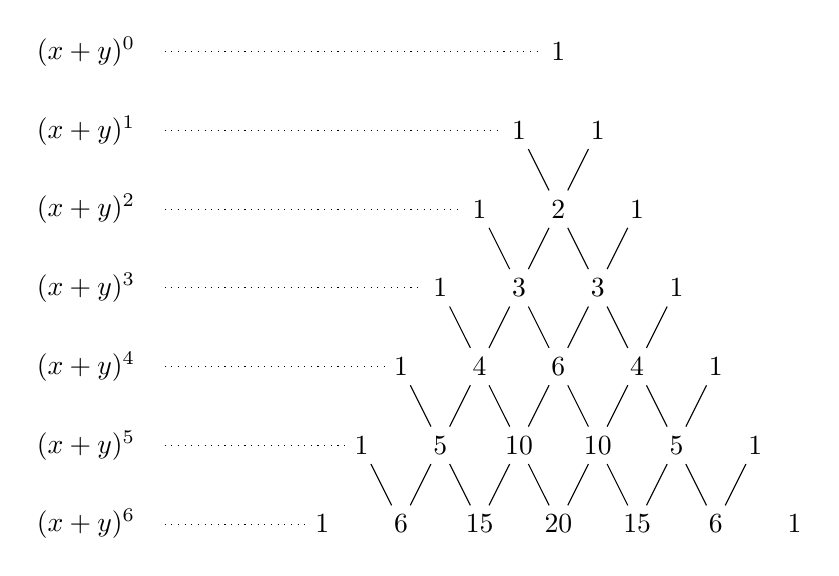
\begin{tikzpicture}
\foreach \x in {0,1,2,...,6}
{
    \node at (0,-\x){$(x+y)^{\x}$};
}
\foreach \x/\y in {3/1, 4/6, 5/15, 6/20, 7/15, 8/6, 9/1}
{
    \node (A\x) at (\x,-6){\y};
}
\foreach \x/\y in {3/1, 4/5, 5/10, 6/10, 7/5, 8/1}
{
    \node (B\x) at (\x+.5,-5){\y};
}
\foreach \x/\y in {3/1, 4/4, 5/6, 6/4, 7/1}
{
    \node (C\x) at (\x+1,-4){\y};
}
\foreach \x/\y in {3/1, 4/3, 5/3, 6/1}
{
    \node (D\x) at (\x+1.5,-3){\y};
}
\foreach \x/\y in {3/1, 4/2, 5/1}
{
    \node (E\x) at (\x+2,-2){\y};
}
\foreach \x/\y in {3/1, 4/1}
{
    \node (F\x) at (\x+2.5,-1){\y};
}
\node (G) at (6,0){1};

\draw(F3)--(E4)--(F4);
\draw(E3)--(D4)--(E4)--(D5)--(E5);
\draw(D3)--(C4)--(D4)--(C5)--(D5)--(C6)--(D6);
\draw(C3)--(B4)--(C4)--(B5)--(C5)--(B6)--(C6)--(B7)--(C7);
\draw(B3)--(A4)--(B4)--(A5)--(B5)--(A6)--(B6)--(A7)--(B7)--(A8)--(B8);

\draw[dotted](1,0)--(G);
\draw[dotted](1,-1)--(F3);
\draw[dotted](1,-2)--(E3);
\draw[dotted](1,-3)--(D3);
\draw[dotted](1,-4)--(C3);
\draw[dotted](1,-5)--(B3);
\draw[dotted](1,-6)--(A3);


\end{tikzpicture}
\end{center}
表中每行两端都是1,而且除1以外的每一个数都等于它肩上两个数的和,这个表叫做杨辉三角,它首先载于我国宋朝数学家杨辉1261年所著的《详解九章算法》一书.
















































































































































\section*{复习题二}
\begin{enumerate}
    \item 解不等式:
\begin{multicols}{2}
\begin{enumerate}[(1)]
    \item $2<\frac{\perm{m+1}{m+1}}{\perm{m-1}{m-1}}\le 42$
    \item $x\perm{3}{8}<\perm{3}{x}$
\end{enumerate}
\end{multicols}

\item 求证:
\begin{enumerate}[(1)]
    \item $1!+2\cdot 2!+3\cdot 3!+\cdots+n\cdot n!=(n+1)!-1$
    
    (提示:$n\cdot n!=(n+1)!-n!$)

\item $\comb{m}{n-1}+\comb{m}{n-2}+\comb{m}{n-3}+\cdots+\comb{m}{m+1}+\comb{m}{m}=\comb{m+1}{n}$
\end{enumerate}

\item \begin{enumerate}[(1)]
    \item 已知$\frac{1}{\comb{m}{5}}-\frac{1}{\comb{m}{6}}=\frac{1}{10\cdot\comb{m}{1}}$,求$\comb{m}{8}$
    \item 已知$\frac{\comb{m-1}{n}}{2}=\frac{\comb{m}{n}}{3}=\frac{\comb{m+1}{n}}{4}$,求$n$与$m$.
\end{enumerate}

\item 用数字0, 1, 2, 3, 4, 5组成没有重复数字的数:
\begin{enumerate}[(1)]
\item 能够组成多少个六位奇数?
\item 能够组成多少个大于201345的自然数? 
\end{enumerate}

\item 8个不同的元素排成一行:
\begin{enumerate}[(1)]
 \item 其中某2个元素要排在一起,有多少种排法?
\item 其中某2个元素不排在一起,有多少种排法?
\item 其中某4个元素要排在一起,另外4个元素也要排在一起,有多少种排法?  
\end{enumerate}

\item 书架上有4本不同的数学书,5本不同的物理书,3本不同的化学书,全部竖起排成一排,如果不使同类的书分开,一共有多少种排法?
\item 从1到9这九个数字每次取出5个数字:
\begin{enumerate}[(1)]
\item 可以组成多少个能被25整除的五位数?
\item 可以组成多少个小于98000的五位数?
\item 可以组成多少个五位偶数?
\item 可以组成多少个奇数位是奇数,偶数位是偶数的五位数?   
\end{enumerate}

\item \begin{enumerate}[(1)]
    \item 一个集合由8个不同的元素组成,这个集合中3个元素的子集有几个?
    \item 一个集合由5个不同的元素组成,其中含1个,2个,3个,4个元素的子集共有几个?
\end{enumerate}

\item \begin{enumerate}[(1)]
\item 平面内有$n$条直线,其中没有两条互相平行,也没有三条相交于一点,一共有多少个交点?
\item 空间有$n$个平面,其中没有两个互相平行,也没有三个相交于一直线,一共有多少条交线?
\item 平面有两组平行线,一组$m$条,另一组$n$条,这两组平行线相交,可以构成多少个平行四边形?
\item 空间有三组平行平面,第一组有$m$个,第二组有$n$个,第三组有$\ell$个,不同组的平面都相交,可以构成多少个平行六面体?
\end{enumerate}

\item 一个班有48名学生,分成六排,每排六人
\begin{enumerate}[(1)]
\item 问:有多少种不同坐法?
\item 若有2人必须坐在前排,3人必须在最后一排,有多少种不同的坐法?
\end{enumerate}

\item 由0至9这10个数字组成的没有重复数字的九位数字有多少个?其中能被3整除的有多少个?
\item 有$n+1$件不同的奖品,全部赠给$n$个先进学生代表.如果每人至少得到一件,有多少种不同的赠送方法?
\item \begin{enumerate}[(1)]
    \item 求$\left(9x-\frac{1}{\sqrt[3]{x}}\right)^{10}$展开式的常数项;
    \item 求$(1+x+x^2)(1-x)^{10}$展开式中$x^4$的系数;
    \item 求$(1-x)^{11}+x(1-2x)^{10}-x^2(1-3x)^9$展开式中$x^5$的系数;
    \item 求$(1+2x-3x^2)^6$展开式中$x^5$的系数;
    \item 求$(x^{-1}-1+x)^5$展开式里不含$x$的项.
\end{enumerate}
\item \begin{enumerate}[(1)]
    \item 用二项式定理证明$55^{55}+9$能被8整除;
    \item 用二项式定理求$89^{10}$除以88的余数.
\end{enumerate}

\item 证明:$(1+x)^{2n}$展开式中$x^n$的系数等于$(1+x)^{2n-1}$展开式中$x^n$的系数的2倍.
\item 已知$\left(\sqrt{x}+\frac{1}{\sqrt[3]{x}}\right)$展开式的系数之和比$(a+b)^{2n}$展开式的系数之和小240,求:
\begin{enumerate}[(1)]
    \item $\left(\sqrt{x}+\frac{1}{\sqrt[3]{x}}\right)$展开式的第三项:
    \item $(a+b)^{2n}$展开式的中间项.
\end{enumerate}

\item 已知$(1+x)^n$展开式里连续三项系数的比是3:8:14,求展开式里系数最大的项.
\item 已知$\left(\sqrt[3]{x^{-2}}+x^2\right)^{2n}$的展开式的系数之和比$\left(\sqrt[3]{x^{-2}}+x^2\right)^{n}$的展开式的系数之和大992,求$\left(\sqrt[3]{x^{-2}}-x^2\right)^{n}$的展开式里含$x^{\tfrac{4}{3}}$项的系数.

\item 证明:
\begin{enumerate}[(1)]
    \item $\sum\limits^n_{k=0}\left(\comb{k}{n}\right)^2=\frac{(2n)!}{n!\cdot n!}$
    \item $\comb{0}{n}\comb{k}{m}+\comb{1}{n}\comb{k-1}{m}+\cdots+\comb{k}{n}\comb{0}{m}=\comb{k}{n+m}$
    \item $\left(\comb{0}{n}-\comb{2}{n}+\comb{3}{n}+\cdots\right)^2+ \left(\comb{1}{n}-\comb{3}{n}+\comb{5}{n}+\cdots\right)^2=\comb{0}{n}+\comb{1}{n}+\comb{2}{n}+\cdots+\comb{n}{n}$
\end{enumerate}

\item 在$(a-3b)^{35}$的展开式中第几项的系数的绝对值最大?
\end{enumerate}

